\documentclass{article}
\usepackage[final,nonatbib]{aaj2026}
\providecommand{\affilmark}[1]{\textsuperscript{#1}}
\providecommand{\affiliations}[1]{}
\providecommand{\correspondence}[1]{}
\usepackage[utf8]{inputenc}
\usepackage[T1]{fontenc}
\usepackage[backend=biber,style=ieee,sorting=none]{biblatex}
\addbibresource{refs.bib}
\usepackage{booktabs}
\usepackage{amsmath}
\usepackage{amssymb}
\usepackage{graphicx}
\usepackage{float}
\usepackage{placeins}
\usepackage[hidelinks]{hyperref}
\graphicspath{{figures/}}
\renewcommand{\thesection}{S\arabic{section}}
\renewcommand{\thetable}{S\arabic{table}}
\renewcommand{\thefigure}{S\arabic{figure}}
\renewcommand{\theequation}{S\arabic{equation}}

\title{Supplementary Material: Patient-Specific Lumped-Parameter Model for Quantifying Shunt Flow and Predicting Post-Closure Hemodynamics in Pediatric Ventricular Septal Defect}
\author{Katili, Subagyo, Dzakiyah, Irnadiastputri, Azwani}
\affiliations{}
\correspondence{puspita.katili@ui.ac.id}

\begin{document}
\maketitle

% Moved from the main text on the supervisor's instruction (2026-09-26):
% the run-to-run repeats (S1) and the practical identifiability audit (S2).
% Text is the authors' own, with cross-references adapted.

\section{Run-to-run repeats of the calibration pipeline}
\label{sec:S-repeats}

\subsection{Method}
The complete pipeline was executed three times with the multi-start seeds 101, 202 and 303, fixed in advance, with clinical inputs and all other settings held constant. The seed enters only through the scrambling of starting points 2--6; starting point 1 is deterministic. All three runs are reported.

\subsection{Result}
The three runs returned the same accepted parameter set, so the pipeline is exactly reproducible under the seeds tested. The reason is visible in the multi-start record (Table~\ref{tab:S-multistart}): the clinically seeded starting point is deterministic and is not affected by the seed, it was the only start with no hard-target failure and the lowest governed error in runs 101 and 202, and it won the lexicographic selection in all three runs. The seed changes only the five scrambled starting points.

Variability therefore exists between starting points rather than between runs. Across the 18 starts, the governed RMSE ranged from 0.0909 to 0.1509. One scrambled start in run 303 reached 0.0909, below the accepted value of 0.1047, but failed one hard target and was rejected by the selection rule. This is the intended behaviour of the rule, and it means the reported result is not the lowest error attained, but the lowest error attained without a hard-target failure.

Because the accepted candidate does not vary, the three repeats do not quantify uncertainty. The measurement-noise simulation of the main text is the analysis intended for that purpose.

\begin{table}[H]
\centering\small
\caption{Governed RMSE of the six starting points in each run, with the number of hard-target failures and gate failures in parentheses. The selected start is in bold.}
\label{tab:S-multistart}
\begin{tabular}{lccc}
\toprule
\textbf{Start} & \textbf{Run 101} & \textbf{Run 202} & \textbf{Run 303} \\
\midrule
Clinically seeded & \textbf{0.1047 (0, 2)} & \textbf{0.1047 (0, 2)} & \textbf{0.1047 (0, 2)} \\
Sobol' 1 & 0.1509 (1, 5) & 0.1509 (1, 5) & 0.1509 (1, 5) \\
Sobol' 2 & 0.1165 (1, 4) & 0.1288 (1, 3) & 0.1209 (1, 3) \\
Sobol' 3 & 0.1211 (1, 3) & 0.1184 (1, 2) & 0.1509 (1, 5) \\
Sobol' 4 & 0.1345 (0, 2) & 0.1392 (0, 2) & 0.1340 (1, 4) \\
Sobol' 5 & 0.1229 (0, 2) & 0.1509 (1, 5) & 0.0909 (1, 2) \\
\bottomrule
\end{tabular}
\end{table}

\section{Practical identifiability}
\label{sec:S-identifiability}

\subsection{Method}
Practical identifiability was assessed at the calibrated operating point from the scaled sensitivity matrix~\cite{Pope2009,Olufsen2013}
\begin{equation}
S_{ij} = \frac{\partial y_i}{\partial \theta_j}\,\frac{\theta_j}{\sigma_i},
\end{equation}
with $\sigma_i$ the declared measurement uncertainty of target $i$. Parameters with small column norms are weakly constrained; pairs with $|\rho| \ge 0.9$ between columns were flagged as collinear. The condition number $\mathrm{cond}(S)$ was evaluated for every subset of size $k \le p$ and the best-conditioned subset at each size reported as a candidate reduced set~\cite{vanOsta2020}. Subsets were scored by linear algebra alone, without re-simulation or recalibration.

\subsection{Result}
With 9 governed targets and 7 fitted parameters the pre-closure problem has 2 degrees of freedom. At the calibrated operating point, $\mathrm{cond}(S)$ of the full seven-parameter set was 61.9, identical in all three runs. No parameter pair was collinear at the $|\rho| \ge 0.9$ criterion; the strongest correlation was $-0.73$ between the pulmonary resistance scale and $C_{\mathrm{SAR}}$, followed by $+0.51$ between the systemic resistance scale and $R_{\mathrm{SVEN}}$. The weakest column was $C_d$ (norm 3.72), followed by $R_{\mathrm{SVEN}}$ (6.56); the pulmonary resistance scale was the best-constrained (27.6).

Conditioning improved sharply on removal of one parameter (Table~\ref{tab:S-cond}): the best six-parameter subset, which drops $R_{\mathrm{SVEN}}$, had $\mathrm{cond}(S) = 9.68$. The seven-parameter set retained here is therefore the least well-conditioned of the candidates, and is kept because it is the set the screen selected, not because it is the best conditioned. The reduced subsets were scored by linear algebra alone and were not recalibrated; they are reported as candidates for a future run.

\begin{table}[H]
\centering\small
\caption{Best condition number of the scaled sensitivity matrix by subset size ($N = 9$ governed targets). Values are identical in all three runs.}
\label{tab:S-cond}
\begin{tabular}{rrrl}
\toprule
$p$ & dof & $\mathrm{cond}(S)$ & \textbf{Parameters} \\
\midrule
7 & $+2$ & 61.90 & full retained set \\
6 & $+3$ & 9.68 & $R_{\mathrm{sys}}, R_{\mathrm{pul}}, C_{\mathrm{SAR}}, C_{\mathrm{PAR}}, E_{\mathrm{B,RV}}, C_d$ \\
5 & $+4$ & 4.00 & $R_{\mathrm{SVEN}}, C_{\mathrm{SAR}}, C_{\mathrm{PAR}}, E_{\mathrm{B,RV}}, C_d$ \\
4 & $+5$ & 2.65 & $R_{\mathrm{SVEN}}, C_{\mathrm{PAR}}, E_{\mathrm{B,RV}}, C_d$ \\
3 & $+6$ & 1.72 & $C_{\mathrm{SAR}}, C_{\mathrm{PAR}}, E_{\mathrm{B,RV}}$ \\
2 & $+7$ & 1.07 & $C_{\mathrm{PAR}}, E_{\mathrm{B,RV}}$ \\
\bottomrule
\end{tabular}
\end{table}

\section{Objective function weights}
\label{sec:S-weights}
Table~\ref{tab:S-weights} lists the target weights $w_k$ and the term weights of the objective function (main-text Eq.~10) as used in the reported run. Target weights are the product of a default weight (1.5 for primary targets, with class-specific minima) and a patient-specific multiplier.

\begin{table}[H]
\centering\small
\caption{Weights of the objective function in the reported calibration.}
\label{tab:S-weights}
\begin{tabular}{llr}
\toprule
\textbf{Term} & \textbf{Quantity} & \textbf{Weight} \\
\midrule
Hard, direct ($\mathcal{H}^{*}$, tolerance 0.05) & mean PA pressure & 1.35 \\
 & $Q_p/Q_s$ & 1.65 \\
Hard, coupled systemic term $J_{\mathrm{sys}}$ & mean RA pressure; mean arterial pressure; $Q_s$ & 1.80; 2.03; 3.24 \\
Soft ($\mathcal{S}$, tolerance 0.10) & PA systolic; PA diastolic & 0.50; 0.45 \\
 & RFA systolic; RFA diastolic & 1.40; 1.30 \\
 & shunt flow & 0.80 \\
$J_{\mathrm{shape}}$ & shunt flow-consistency term & 0.15 \\
Gate hinge & $\lambda_{\mathrm{g}}$, gate 10\% & 20 \\
Prior & $\lambda_{\mathrm{p}}$ (stages A--D, F); stage E & 0.375; 2.25 \\
Bound proximity & $\lambda$ (stages A--D, F); stage E & 17; 120 \\
Physiological range & soft; hard band & 50; 400 \\
\bottomrule
\end{tabular}
\end{table}

\section{Supplementary figures}

\begin{figure}[H]
\centering
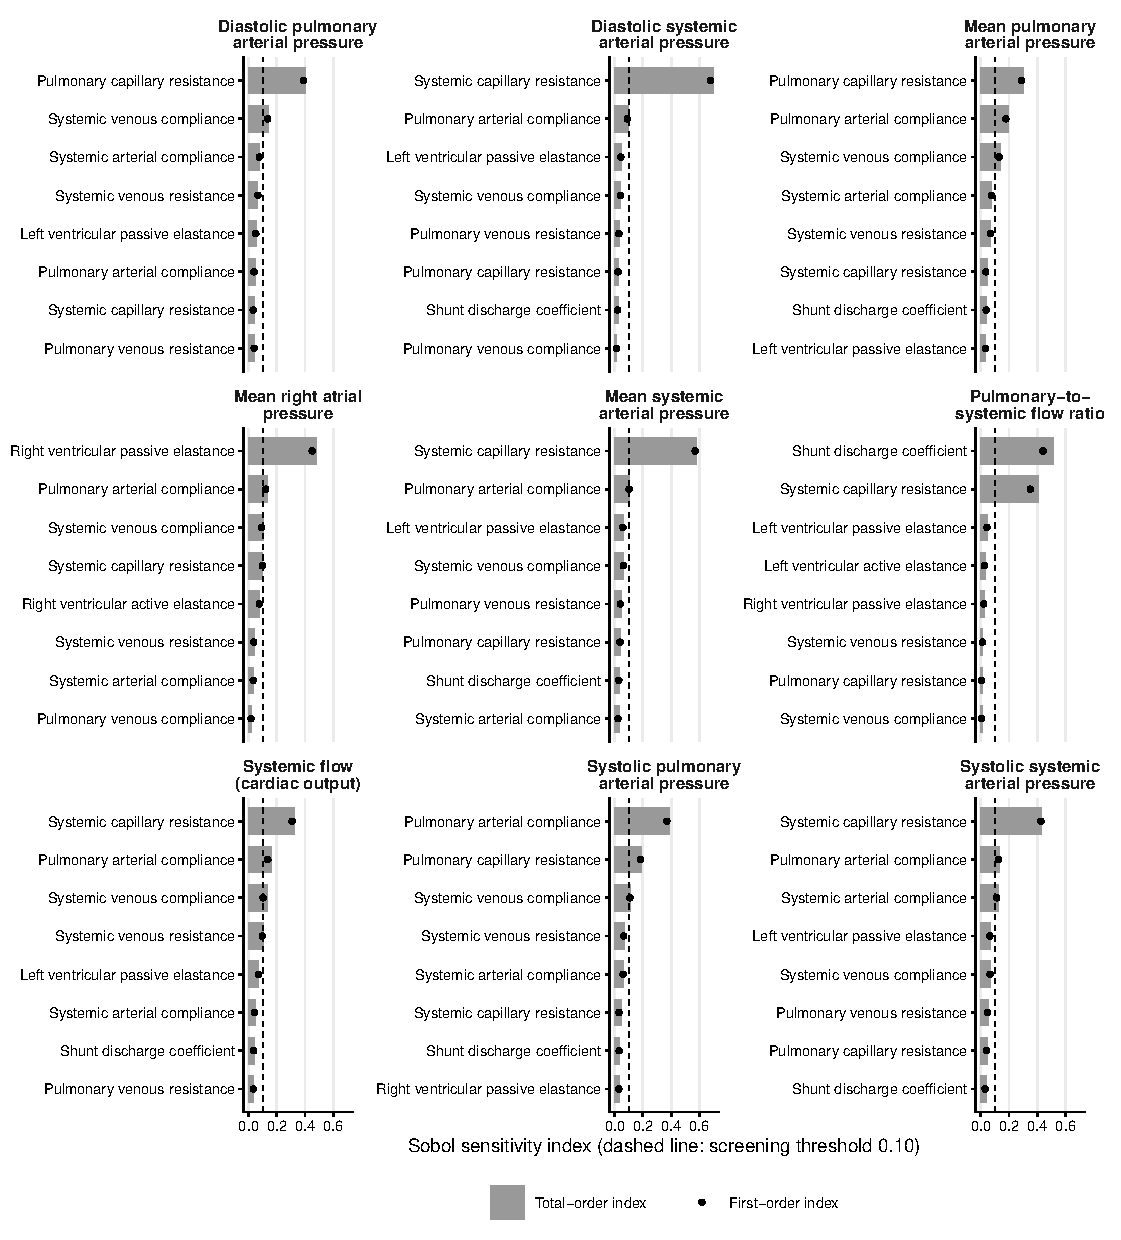
\includegraphics[width=0.95\linewidth]{F01_gsa_tornado_screening.pdf}
\caption{Total-order (bars) and first-order (points) Sobol' indices at the scaled baseline for each governed target, eight largest parameters per target. Dashed line: retention threshold 0.10.}
\label{fig:S-tornado-initial}
\end{figure}

\begin{figure}[H]
\centering
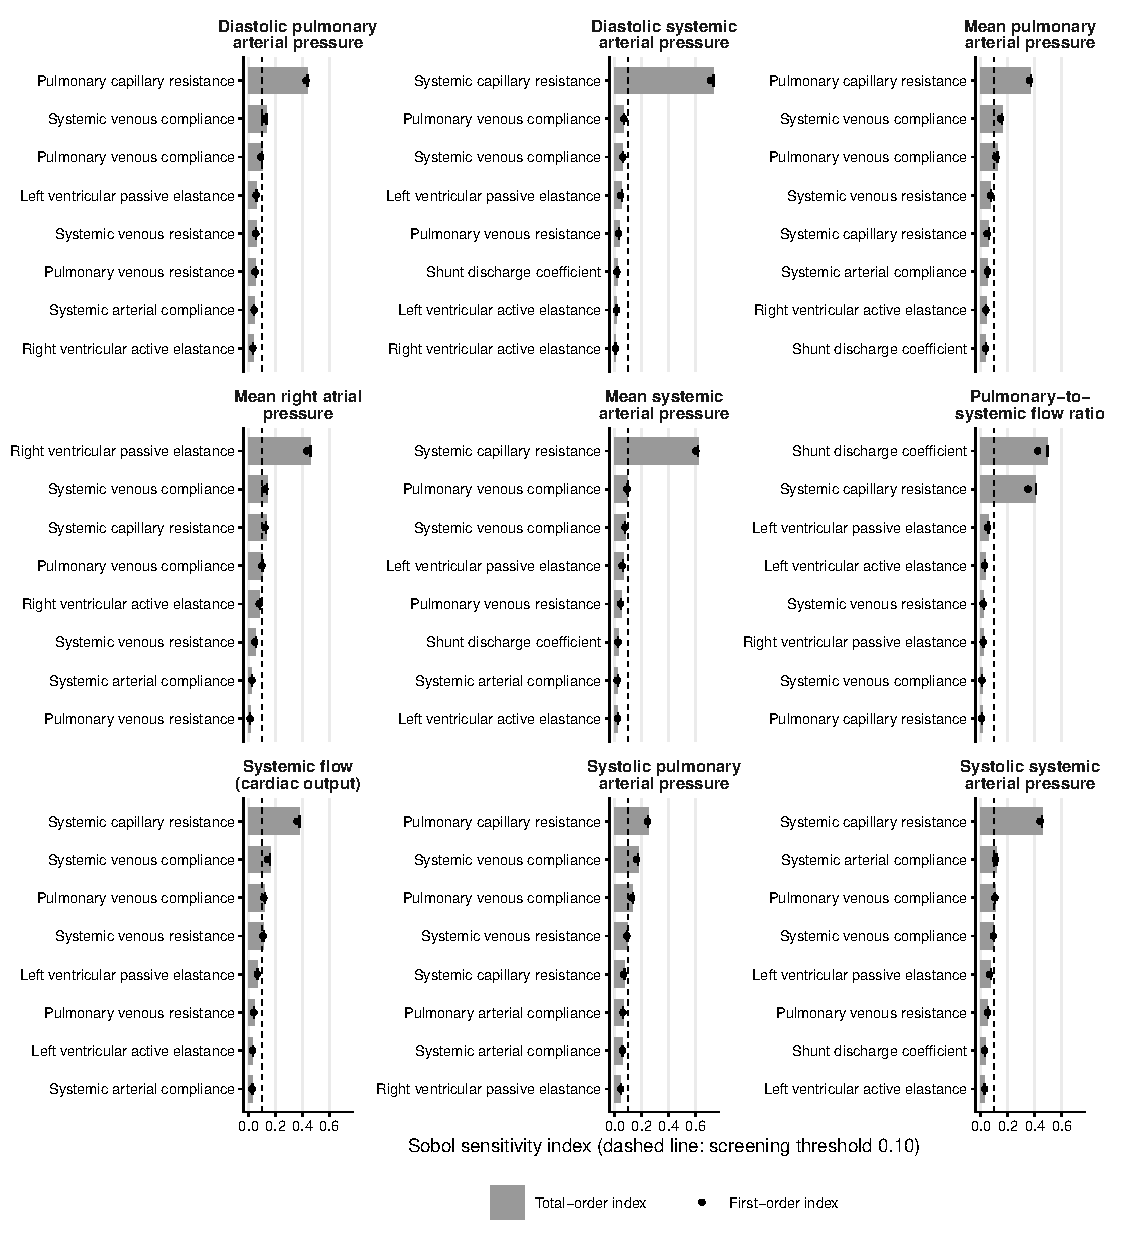
\includegraphics[width=0.95\linewidth]{F02_gsa_tornado_calibrated.pdf}
\caption{Sobol' indices repeated at the calibrated operating point (mean and range over the three runs).}
\label{fig:S-tornado-final}
\end{figure}

\begin{figure}[H]
\centering
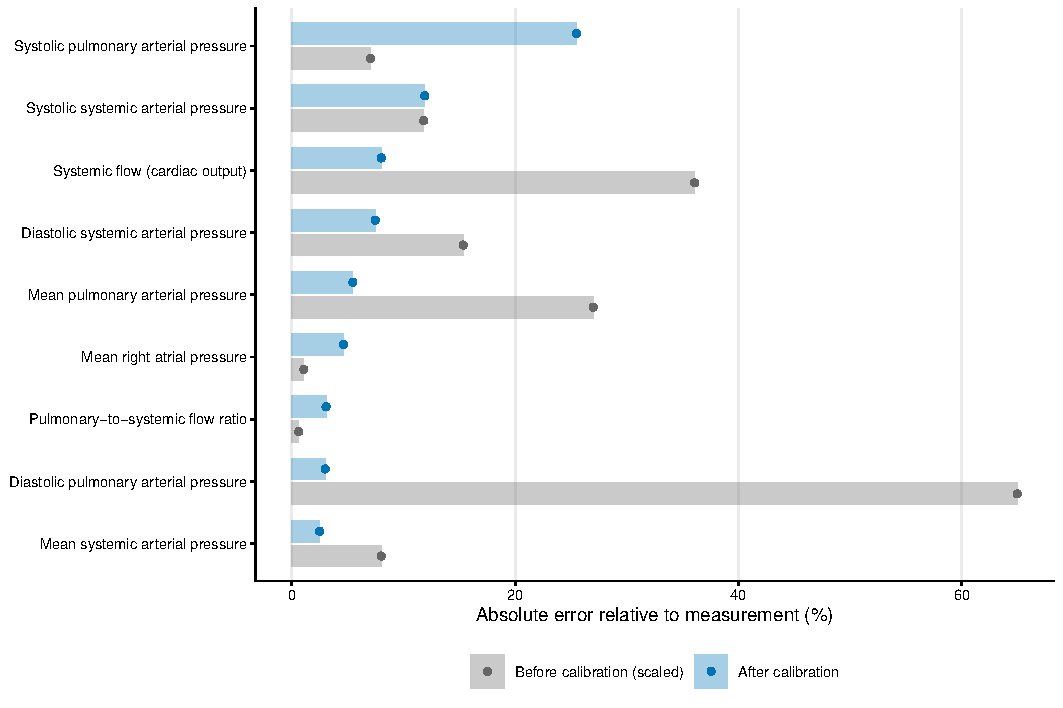
\includegraphics[width=0.9\linewidth]{F03_calibration_before_after.pdf}
\caption{Absolute relative error of each governed target at the scaled baseline and after calibration. Dashed line: 10\% acceptance gate.}
\label{fig:S-before-after}
\end{figure}

\printbibliography
\end{document}
